\id{МРНТИ: 65.01.84}{https://doi.org/10.58805/kazutb.v.2.27-968}

\begin{articleheader}
\sectionwithauthors{Г.К. Хакимов, М. Б. Икрами}{ТРАНСФОРМАЦИЯ «ЗЕЛЕНЫХ» ТЕХНОЛОГИЙ В УСЛОВИЯХ ЦИФРОВИЗАЦИИ
ПИЩЕВОЙ ПРОМЫШЛЕННОСТИ}

{\bfseries
Г.К. Хакимов\alink{https://orcid.org/0009-0006-0736-5266}\textsuperscript{\envelope },
М. Б. Икрами\alink{https://orcid.org/0009-0000-2072-9677}
}
\end{articleheader}

\begin{affiliation}
Технологический университет Таджикистана, Душанбе, Таджикистан

\raggedright \textsuperscript{\envelope }Корреспондент автор: gafurjon-68@mail.ru
\end{affiliation}

В данной научной статье рассматриваются процессы трансформации пищевой
промышленности Республики Таджикистан в контексте внедрения «зеленых»
технологий и цифровизации. Проведен анализ ключевых проблем отрасли,
включая рост выбросов CO₂, дефицит продовольствия и экологическую
нагрузку производств. В работе применены методы статистического анализа,
сравнительного анализа международного опыта внедрения устойчивых
технологий и аналитические подходы к оценке эффективности цифровизации.
Представлены динамические показатели внедрения «зеленых» технологий и
цифровых решений в пищевой промышленности Таджикистана за 2013--2023
гг., а также сравнительный анализ с ведущими мировыми странами, такими
как Германия и Франция. В заключении даны рекомендации по ускоренной
модернизации отрасли и внедрению стратегий устойчивого развития.

{\bfseries Ключевые слова:} тренд, пищевая промышленность,
индустриализация, «зеленая» экономика, колаборация, продовольственная
безопасность, энергоэффективность, возобновляемые источники энергии,
конкурентоспособность.

\begin{articleheader}
{\bfseries ЦИФРЛАНДЫРУ ЖАҒДАЙЫНДА АЗЫҚ-ТҮЛІК ӨНЕРКӘСІБІНДЕГІ «ЖАСЫЛ» ТЕХНОЛОГИЯЛАРДЫ ТРАНСФОРМАЦИЯЛАУ}

{\bfseries
Г.К.Хакимов\textsuperscript{\envelope },
М. Б.Икрами
}
\end{articleheader}

\begin{affiliation}
Тәжікстан Технологиялық университеті, Душанбе, Тәжікстан,

e-mail: gafurjon-68@mail.ru
\end{affiliation}

Бұл ғылыми мақалада Тәжікстан Республикасының азық-түлік өнеркәсібіндегі
«жасыл» технологиялар мен цифрлықтандыру үдерістерінің трансформациясы
қарастырылады. Саланың негізгі мәселелері, соның ішінде CO₂
шығарындыларының өсуі, азық-түлік тапшылығы және өндірістің экологиялық
жүктемесі талданды. Зерттеуде статистикалық талдау әдістері, тұрақты
технологияларды енгізудің халықаралық тәжірибесін салыстырмалы талдау
және цифрлықтандыру тиімділігін бағалау әдістері қолданылды.2013-2023
жылдар аралығында Тәжікстанның азық-түлік өнеркәсібінде «жасыл»
технологиялар мен цифрлық шешімдерді енгізудің динамикалық көрсеткіштері
ұсынылып, Германия мен Франция сияқты әлемдік жетекші елдермен
салыстырмалы талдау жасалды. Қорытындыда саланы жедел жаңғырту және
тұрақты даму стратегияларын енгізу бойынша ұсыныстар берілді.

{\bfseries Түйін сөздер}: тренд, азық-түлік өнеркәсібі, индустрияландыру,
«жасыл» экономика, коллаборация, азық-түлік қауіпсіздігі, энергия
тиімділігі, жаңартылатын энергия көздері, бәсекеге қабілеттілік.

\begin{articleheader}
{\bfseries TRANSFORMATION OF "GREEN" TECHNOLOGIES IN THE CONDITIONS OF DIGITALIZATION OF THE FOOD INDUSTRY}

{\bfseries
G.K Khakimov\textsuperscript{\envelope },
M.B.Ikrami
}
\end{articleheader}

\begin{affiliation}
Technological University of Tajikistan, Dushanbe, Republic of Tajikistan,

e-mail: gafurjon-68@mail.ru
\end{affiliation}

This scientific article examines the processes of transformation of the
food industry in the Republic of Tajikistan in the context of the
introduction of ' green'{} technologies
and digitalization. An analysis of key industry issues, including the
growth of CO₂ emissions, food shortages, and the environmental impact of
production, was conducted. The study employs methods of statistical
analysis, comparative analysis of international experience in the
implementation of sustainable technologies, and analytical approaches to
assessing the effectiveness of digitalization. Dynamic indicators of the
introduction of ' green'{} technologies
and digital solutions in Tajikistan's food industry for the period
2013--2023 are presented, along with a comparative analysis with leading
global countries such as Germany and France. The conclusion provides
recommendations for accelerating industry modernization and implementing
sustainable development stra\-tegies.

{\bfseries Keywords:} trends, food industry, industrialization,
' green' economy, collaboration, food
security, energy efficiency, renewable energy sources, competitiveness.

\begin{multicols}{2}
{\bfseries Введение.} В условиях трансформации экономики реальный сектор --
промышленность - переживает значительные изменения, связанные с
модернизацией и диверсификацией. Промышленные предприятия играют
ключевую роль в экономике государства, формируя более 26\% ВВП страны
{[}1{]}. При этом развитие отрасли сопровождается как экономическими,
так и экологическими вызовами, связанными с индустриализацией и
техногенным воздействием на окружающую среду.

На глобальном уровне устойчивое развитие промышленности является
стратегическим приоритетом, однако индустриализация сопровождается рядом
негативных последствий, включая деградацию экосреды городов, рост
выбросов CO₂, загрязнение тяжелыми металлами и повышение заболеваемости
населения {[}2{]}. Среди ключевых вызовов современной промышленности
можно выделить:

- ухудшение экологической ситуации в мегаполисах;

- высокий уровень промышленных выбросов СО₂ и иных загрязнителей;

- рост заболеваний, связанных с экологическими факторами (ОРВИ,
гипертония, кожные заболевания и др.);

- загрязнение окружающей среды тяжелыми металлами и токсичными отходами;

- нехватку квалифицированных кадров в промышленных секторах;

- недостаточное сотрудничество между вузами и промышленными
предприятиями;

- низкую инвестиционную активность в стратегически важные отрасли
{[}3{]}.

В пищевой промышленности данные вызовы приобретают особое значение, так
как производство продуктов питания напрямую влияет на здоровье
населения. Основные проблемы данной отрасли включают:

1. Чрезмерная очистка сырья, приводящая к потере жизненно важных
нутриентов (например, удаление витаминов группы B при переработке
пшеницы, фосфатидов из растительных масел) {[}4{]}.

2. Использование пищевых добавок для улучшения характеристик продукции,
не всегда безопасных для здоровья {[}5{]}.

3. Загрязнение окружающей среды отходами пищевой промышленности,
содержащими тяжелые металлы и токсичные соединения {[}6{]}.

4. Дефицит продовольствия, особенно в развивающихся странах, и снижение
потребления важных продуктов (мясо, рыба, овощи, фрукты), приводящее к
"скрытому голоду" -- нехватке микроэлементов и нутриентов {[}7{]}.

Для решения указанных проблем необходим переход к "зеленым технологиям"
-- экологически ориентированным методам производства, снижающим
негативное воздействие на окружающую среду. В 2008 году ООН инициировала
программу ``Green Economy Initiative'', направленную на стимулирование
развития экологически чистых и энергоэффективных технологий во всех
секторах экономики, включая промышленность, сельское хозяйство и
управление отходами {[}8{]}.

Таким образом, трансформация пищевой промышленности с учетом принципов
"зеленой экономики" требует научного обоснования и внедрения
инновационных технологий, обеспечивающих безопасность и
ресурсосбережение на всех этапах производства. Введение новых
технологических процессов, использование возобновляемых источников
энергии и разработка функциональных продуктов, обогащенных полезными
компонентами, являются приоритетными направлениями устойчивого развития
отрасли {[}9{]}.

{\bfseries Материалы и методы.} В рамках исследования использованы методы
статистического анализа, сравнительный анализ международного опыта
внедрения «зеленых» технологий, а также аналитические подходы к оценке
эффективности цифровизации в пищевой промышленности.

\emph{{\bfseries Методы статистического анализа.}} Статистический анализ
был проведен на основе официальных данных о выбросах CO₂, уровня
внедрения «зеленых» технологий и цифровизации в пищевой промышленности
Республики Таджикистан. Основные параметры исследования включали
(таблица 1):

- динамику выбросов CO₂ в пищевой промышленности за 2013- 2023 гг.;

- долю предприятий, использующих возобновляемые источники энергии;

- долю цифровизированных предприятий в отрасли.
\end{multicols}

\tcap{Таблица 1 - Динамика внедрения «зеленых» технологий в пищевой промышленности Таджикистана}
\begin{longtblr}[
  label = none,
  entry = none,
]{
  width = \linewidth,
  colspec = {Q[48]Q[367]Q[273]Q[246]},
  cells = {c},
  hlines,
  vlines,
}
\textbf{Год} & \textbf{Доля			предприятий, использующих «зеленые»			технологии (\%)} & \textbf{Доля			цифровизированных предприятий (\%)} & \textbf{Среднегодовой			рост выбросов CO₂ (\%)}\\
2013 & 15 & 5 & 2.1\\
2015 & 20 & 10 & 2.4\\
2017 & 28 & 18 & 2.6\\
2019 & 35 & 26 & 2.9\\
2021 & 40 & 34 & 3.2\\
2023 & 45 & 42 & 3.5
\end{longtblr}

\begin{multicols}{2}
Анализ представленных данных демонстрирует устойчивую тенденцию роста
доли предприятий, использующих «зеленые» технологии в пищевой
промышленности Таджикистана. В 2013 году только 15\% предприятий отрасли
использовали экологически чистые технологии, тогда как к 2023 году этот
показатель увеличился до 45\%, что свидетельствует о постепенной
трансформации отрасли в направлении устойчивого развития.

Среднегодовой темп роста данного показателя за десятилетний период
составил около 3\% в год, что указывает на позитивную динамику, но
недостаточную для быстрого перехода на экологически чистое производство.
В странах с более развитой экологической политикой аналогичный
показатель превышает 60--70\%, что свидетельствует о наличии
значительных резервов для роста.

Факторы, влияющие на рост внедрения «зеленых» технологий в Таджикистане:

- Развитие законодательной базы. Введение новых норм и стандартов
стимулирует предприятия к переходу на устойчивые технологии.

- Инвестиции в возобновляемые источники энергии. В последние годы
увеличивается доля предприятий, использующих солнечную и
гидроэнергетику.

- Поддержка со стороны международных организаций. Различные программы
содействия «зеленой» экономике помогают привлекать инвестиции в данную
сферу.
Одновременно с внедрением «зеленых» технологий наблюдается рост уровня
цифровизации предприятий отрасли. В 2013 году лишь 5\% предприятий
использовали цифровые решения, однако к 2023 году этот показатель
увеличился до 42\%. Данный рост обусловлен следующими факторами:

- внедрение автоматизированных систем управления производством;

- развитие цифровых платформ для логистики и контроля качества
продукции;

- использование «умных» датчиков и аналитики больших данных для
мониторинга состояния производства.

{\bfseries Обсуждение и результаты}. Средний темп роста цифровизации
составил ≈4\% в год, что является положительной тенденцией, однако
уровень цифровизации все еще отстает от мировых стандартов, где данный
показатель в пищевой промышленности может достигать 50-70\%. Дальнейшее
развитие цифровых решений в отрасли позволит повысить эффективность
использования ресурсов, сократить издержки и минимизировать отходы.

Несмотря на увеличение доли предприятий, использующих «зеленые»
технологии и цифровые решения, уровень выбросов углекислого газа
продолжает расти. В 2013 году среднегодовой темп роста выбросов CO₂
составлял 2,1\%, тогда как в 2023 году он достиг 3,5\%. Это
свидетельствует о недостаточной эффективности предпринимаемых мер по
сокращению загрязнений.

Факторы, способствующие росту выбросов CO₂:

- рост производственных мощностей пищевой промышленности;

- ограниченная доступность современного экологического оборудования;

- низкий уровень энергоэффективности существующих предприятий;

- задержки в модернизации старых промышленных объектов.
\end{multicols}

\tcap{Таблица 2 - Международный опыт внедрения «зеленых» технологий в пищевой промышленности}
\begin{longtblr}[
  label = none,
  entry = none,
]{
  width = \linewidth,
  colspec = {Q[100]Q[250]Q[433]Q[171]},
  cells = {c},
  hlines,
  vlines,
}
\textbf{Страна} & \textbf{Уровень			внедрения «зеленых» технологий (\%)} & \textbf{Основные			меры} & \textbf{Снижение			выбросов CO₂ (\%)}\\
Германия & 75 & {
			Энергоэффективные
			технологии, утилизация отходов,
			возобновляемые
			\\
			источники
			энергии
		} & 12\\
Франция & 68 & Оптимизация
			технологических процессов, модернизация
			предприятий, снижение углеродного
			следа & 10\\
Таджик\-истан & 45 & Внедрение
			солнечной и гидроэнергии, частичная
			модернизация пищевых производств & 5
\end{longtblr}

\begin{multicols}{2}
Таким образом, несмотря на положительные тенденции внедрения устойчивых
технологий и цифровизации, экологическая нагрузка пищевой промышленности
остается значительной. Для достижения реального сокращения выбросов
необходим комплексный подход, включающий:

- ускоренную модернизацию предприятий с заменой устаревшего оборудования
на энергоэффективные установки;

- увеличение инвестиций в возобновляемые источники энергии;

- применение более строгих экологических нормативов и налогов на выбросы.

Анализ представленных данных показывает, что пищевой сектор Таджикистана
активно движется в направлении устойчивого развития.

\emph{{\bfseries Сравнительный анализ международного опыта внедрения
«зеленых» технологий.}}

Для оценки внедрения «зеленых» технологий в пищевой промышленности были
выбраны три страны: Германия, Франция и Таджикистан. Сравнительный
анализ основан на данных по уровням внедрения технологий и их влиянию на
снижение выбросов (таблица 2).

Проведенный сравнительный анализ показывает, что уровень внедрения
«зеленых» технологий в пищевой промышленности значительно варьируется в
зависимости от экономического развития страны, доступности ресурсов и
государственной поддержки. В таблице представлены показатели Германии,
Франции и Таджикистана, отражающие их текущие стратегии и результаты в
области устойчивого производства.

1. Германия: лидер в использовании «зеленых» технологий.

Германия демонстрирует самый высокий уровень внедрения экологически
чистых технологий в пищевой промышленности - 75\% предприятий отрасли
активно используют «зеленые» технологии. Это объясняется следующими
факторами:

- энергоэффективность как государственный приоритет - Германия активно
инвестирует в модернизацию предприятий, внедрение энергоэффективных
решений и использование экологически чистых технологий на всех этапах
пищевого производства;

- расширенная система утилизации и переработки отходов- применяются
технологии вторичной переработки органических отходов, биогазовые
установки, компостирование, что позволяет минимизировать негативное
воздействие на окружающую среду;

- использование возобновляемых источников энергии - многие предприятия
переходят на солнечную, ветровую и биогазовую энергетику, снижая
зависимость от ископаемого топлива;

- жесткие экологические стандарты - в стране действуют строгие
нормативы, регулирующие выбросы парниковых газов, использование воды и
управление отходами.

В результате принятых мер Германия добилась снижения выбросов CO₂ на
12\%, что является одним из лучших показателей среди развитых стран. Это
свидетельствует о высокой эффективности внедренных технологий и строгого
регулирования отрасли.

2. Франция: модернизация пищевых производств для снижения углеродного
следа.

Франция также демонстрирует высокий уровень экологической трансформации
пищевой промышленности - 68\% предприятий используют «зеленые»
технологии. Основные стратегии включают:

- оптимизацию технологических процессов - использование более
энергоэффективных линий производства, интеллектуальных систем управления
и автоматизированных решений позволяет сократить энергопотребление и
минимизировать отходы;

- глубокая модернизация предприятий -- в последние десятилетия
значительные инвестиции направлены на обновление оборудования, что
позволило значительно повысить экологическую безопасность производства;

- программы по снижению углеродного следа -- г осударство активно
стимулирует компании к использованию низкоуглеродных технологий и
компенсирует затраты на внедрение энергоэффективных решений;

- развитие органического сельского хозяйства. Важную роль в пищевой
промышленности Франции играет переход на органическое земледелие, что
снижает нагрузку на почву, водные ресурсы и уменьшает выбросы CO₂.

Благодаря этим мерам уровень выбросов углекислого газа в пищевой
промышленности страны снизился на 10\%, что подтверждает эффективность
комплексного подхода к экологической модернизации отрасли.

3. Таджикистан: начальный этап внедрения устойчивых технологий

В Таджикистане уровень внедрения «зеленых» технологий остается на
относительно низком уровне (45\%), что обусловлено рядом экономических и
технологических факторов. Основные направления экологической
трансформации пищевой промышленности включают:

- использование солнечной и гидроэнергии - Таджикистан обладает
значительным потенциалом возобновляемых источников энергии, особенно
гидроэнергии, что позволяет некоторым предприятиям частично отказаться
от традиционных источников топлива;

- частичная модернизация производственных мощностей - в последние годы
проводится обновление оборудования, однако процесс идет медленными
темпами из-за ограниченного финансирования;

- ограниченные возможности переработки отходов -- в отличие от Германии
и Франции, утилизация и переработка пищевых отходов в стране развиты
слабо, что увеличивает экологическую нагрузку на окружающую среду;

- недостаточный уровень экологического регулирования - в стране только
начинают вводиться законодательные нормы, стимулирующие предприятия к
переходу на «зеленые» технологии.

В результате уровень снижения выбросов CO₂ в пищевой промышленности
Таджикистана составляет всего 5\%, что указывает на необходимость более
активных мер по экологической модернизации отрасли.

Анализ международного опыта показывает, что успешное внедрение «зеленых»
технологий в пищевой промышленности зависит от ряда факторов:

1. Государственной поддержки. В Германии и Франции разработаны детальные
программы субсидирования и налогового стимулирования предприятий,
переходящих на устойчивое производство.

2. Инвестиционной активности. Развитые страны вкладывают значительные
ресурсы в модернизацию пищевой промышленности, в то время как в
Таджикистане этот процесс требует более масштабного финансирования.

3. Развитости инфраструктуры переработки отходов. Высокий уровень
утилизации органических отходов в Германии и Франции способствует
снижению экологической нагрузки, тогда как в Таджикистане этот сегмент
развит недостаточно.

4. Широкого применения возобновляемых источников энергии. Германия и
Франция активно используют солнечную, ветровую и биогазовую
энергетику, что значительно сокращает выбросы CO₂. В Таджикистане пока
только начинается переход на возобновляемую энергетику.

\emph{{\bfseries Аналитические подходы к оценке эффективности
цифровизации.}}

Для оценки эффективности цифровизации пищевой промышленности
Таджикистана были использованы ключевые показатели, такие как:

- уровень автоматизации производственных процессов;

- влияние цифровизации на сокращение затрат и повышение
производительности;

- доля предприятий, использующих умные системы управления.

Цифровизация пищевой промышленности является одним из ключевых
направлений её модернизации, способствующих повышению эффективности
производства, снижению издержек и минимизации негативного воздействия на
окружающую среду. В период с 2013 по 2023 год наблюдается устойчивый
рост доли цифровизированных предприятий в пищевой промышленности
Таджикистана.

Анализ представленных данных показывает, что если в 2013 году уровень
цифровизации составлял 5\%, то к 2023 году он увеличился до 42\%, что
свидетельствует о значительном прогрессе в данном направлении.
Среднегодовой темп роста цифровизации в отрасли составил ≈4\% в год, что
является положительной тенденцией, но при этом данный показатель
остается ниже, чем в ведущих странах, где уровень цифровизации достигает
50-70\%.
\end{multicols}

\begin{figure}[H]
	\centering
	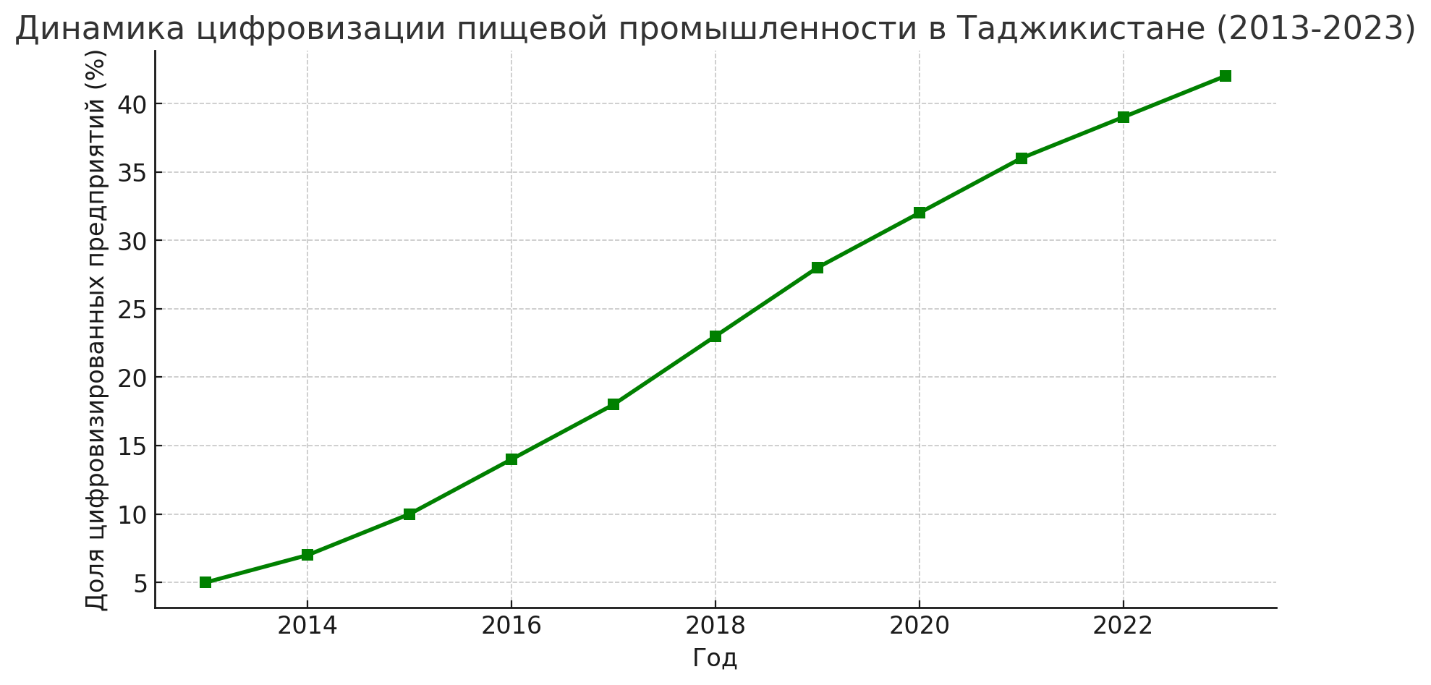
\includegraphics[width=0.8\textwidth]{media/ekon2/image48}
	\caption*{Рис.1 - Динамика цифровизации пищевой промышленности в Таджикистане (2013-2023)}
\end{figure}

\begin{multicols}{2}
График 1 иллюстрирует экспоненциальный рост цифровизации, что
обусловлено несколькими ключевыми факторами:

- увеличением количества автоматизированных производственных линий на
крупных предприятиях;

- внедрением цифровых систем управления качеством и логистикой;

- ростом популярности «умных» датчиков и технологий Интернета вещей
(IoT);

- развитием электронных платформ для управления поставками и продажами.

\emph{{\bfseries Этапы цифровизации}}

2013 - 2017 гг.: Начальный этап цифровизации. В этот период цифровизация
развивалась медленно, так как предприятия только начинали внедрять
информационные технологии в производственные процессы. В 2013 году лишь
5\% предприятий использовали цифровые решения, а к 2017 году этот
показатель достиг 18\%. Основными причинами медленного роста являлись:

- высокая стоимость внедрения цифровых технологий;

- недостаточное количество квалифицированных кадров в сфере
автоматизации и информационных технологий;

- ограниченные инвестиции в модернизацию производства.

2017- 2021 гг.: Активное внедрение цифровых решений. За этот период
наблюдается более быстрый рост уровня цифровизации. В 2019 году доля
цифровизированных предприятий достигла 26\%, а к 2021 году - 34\%.
Ключевыми факторами роста стали:

- развитие государственных программ поддержки цифровой трансформации
промышленности;

- расширение использования автоматизированных систем управления
производством (MES, ERP);

- повышение интереса бизнеса к оптимизации затрат за счёт внедрения
цифровых решений;

2021- 2023 гг.: Ускоренная цифровая трансформация. В этот период уровень
цифровизации вырос с 34\% до 42\%, что указывает на ускорение темпов
внедрения цифровых технологий. В этот период широкое распространение
получили:

- роботизированные линии производства, которые позволили значительно
сократить трудозатраты и повысить точность технологических процессов;

- автоматизированные системы мониторинга выбросов и энергопотребления,
что позволило предприятиям снижать экологическую нагрузку;

- цифровые маркетинговые платформы, позволяющие автоматизировать работу
с клиентами и увеличивать конкурентоспособность.

Анализ динамики цифровизации пищевой промышленности в Таджикистане с
2013 по 2023 год показывает устойчивый рост внедрения цифровых
технологий, что способствует повышению эффективности и
конкурентоспособности отрасли.

\emph{{\bfseries Нормативно - правовая основа для реализации стратегических
целей внедрения ``зеленых'' технологий в Таджикистане.}}

Республика Таджикистан имеет важные предпосылки для внедрения «зеленых
технологий» и превращения экономики в «зеленую». Так, по официальным
данным, преобладающее большинство территории Республики Таджикистан на
93\% состоит из горных регионов, где концентрированы экологически чистые
воды и возобновляемые источники энергии. На территории страны
формируется 64\% водных ресурсов Центральной Азии из более 13 тыс.
ледников и 1000 рек с общим потенциалом 527 млрд. кВт/ч. Электроэнергия
в основном вырабатывается за счет возобновляемых источников энергии.
Этому процессу соответствует благоприятный географический климат страны
с 280 -- 330 солнечными днями и общей интенсивностью солнечного
излучения более 2000 кВт/м, что несомненно благоприятно для
использования солнечной энергии и оно по сравнению с ведущими странами
Евросоюза в 2 раза больше. По официальным расчетным данным общий
потенциал страны составляет около 25,16 кВт/ч в год, что может обеспечит
от 60 - 80\% от общей потребности населения в течение 10 месяцев в году
по всей страны.

Следует отметить, что в Республике Таджикистан (РТ) уже имеется
нормативно - правовая основа для реализации стратегических целей
внедрения ``зеленых'' технологий. Правительством Республики Таджикистан
принят ряд основополагающих законодательных актов, в том числе законы
Республики Таджикистан «О безопасности пищевых продуктов», «Об
обеспеченности населения обогащенными продуктами», принята Стратегия
развития ``зеленой'' экономики в РТ на период 2023-2030 годы
(Постановление Правительства РТ от 30.09.2022г., № 482) и другие
международные правовые акты, признанные Республикой Таджикистан.

Вышеперечисленные нормативно-правовые акты акцентированы на мерах
проведения инстутициональных реформ по всей вертикали власти,
промышленных предприятий и вузов, привлечении внутренных и внешних
инвестиций, внедрении инновационных технологий и всемерное укрепление
международного сотрудничества с ведушими компаниями и вузами в сфере
``зеленой'' экономики, превентивной государственной поддержке научно -
исследовательских работ, связанных с использованием зеленых
ресурсо-энергосберегающих технологий (по приоритетным направлениям) и
отдачей/возвратом затрат.

Реализация правовых актов непосредственно будет способствовать
обеспечиванию устойчивого социально-экономического роста во всех сферах
пищевой промышленности, улучшению экологически благоприятной среды,
повышению уровня жизни и соответственно долголетию жителей страны.

Одним из ключевых задач успешного внедрения «зеленой» технологии с
учетом цифровизации пищевых предприятий, несомненно, является подготовка
высококвалифицированных кадров с адаптированными гибкими знаниями с
учетом требований реалий времени и быстроизменяющиеся рынка труда.
Отраслевые вузы страны обязаны вести политику несомненной диверсификации
структуры управления и организации новых специальностей, отвечающих
требованиям «зеленой» технологии с учетом цифровизации пищевых отраслей.
Колаборативно вести правильную систему работ с ведущими пищевыми
предприятиями, обеспечить устойчивую академическую мобильность
профессорско-преподавательского состава и студентов всех ступеней
образования (бакалавры, магистранты, докторанты PhD) за счет средств
вуза и международных образовательных проектов и фондов (Дурахшандагон,
Эрасмуз+, GIZ, Маски, Фулбрайт и др.), изучение международного
передового опыта с колаборативной разработкой гибких Образовательных
программ с учетом дуального образования. Планирование и обеспечение
устойчивой совместной деятельности цепочки вуз + предприятия с
обеспечением выпуска конкурентной продукции профилактического и
функционального назначения из местных трав и растений, соблюдая
требований обеспечения продовольственной безопасности.

С учетом вышеизложенного, в условиях трансформации «зеленой» технологии
и цифровизации пищевых отраслей наиболее адаптированным вузом страны
является Технологический университет Таджикистана (ТУТ), имеющий богатый
опыт многолетней колаборативной деятельности с ведущими пищевыми
предприятиями страны, вузами Евросоюза и других экономически развитых
стран.

На рынке образовательных услуг ТУТ входит в десятку лучших вузов
Таджикистана и является самым первым (пилотным) вузом по внедрению
кредитной технологии образования и успешно реализуемой поныне с ведущими
вузами стран Евросоюза и Центральной Азии. Имеется взаимные договора с
более 100 вузами стран мира. Пять специальностей вуза имеют
международные сертификаты соответствия качества по Европейским ESG
стандартам.

В условиях цифровизации актуально и важно создание цепочки отношений вуз
+ предприятия, целью которой является систематическое и эффективное
внедрение информационно - коммуникационной технологии по всей цепочке,
включающую подготовку кадров, переработку и производство конкурентной
пищевой продукции, что, соответственно, ведет к повышению
производительности, обеспечению благоприятной мотивационной среды,
оптимизации технологических процессов, контролю за всеми
технологическими процессами производства продукции, уменьшению участия
работников в травмоопасных участках и операциях, дистанционному
управление всеми технологическими процессами, легкости автоматизации и
роботизации всего технологического процесса с учетом складских работ,
легкой и более точной обработке и анализа базы данных, повышения
эффективности и прибыльности предприятия, улучшению социальной и
климатической среды рабочих, легкости адаптации к выпуску ассортиментов
продукций по требованиям «халяль».

Период пандемии четко определил, насколько пищевые предприятия страны
нуждаются к реорганизации и трансформации, и она выявила их наиболее
слабые стороны, подтолкнула на активные действия по оптимизации
производства и внедрению инновационных технологий. Современные цифровые
технологии, внедряемые на пищевые предприятия, предполагают поддерживать
стабильность цепочки технологического производства. Основное внимание
будет обращено на качество готового продукта и их безопасность. С
большой долей вероятности предполагаем, что стандартные требования к
выпуску ассортимента продукций будут ужесточены, потребители более
требовательны, что подталкивает к новым решениям и привлечению новых
ресурсов. Способность подстраиваться к изменчивой и гибкой экономике -
основное качество для таких категорий пищевых предприятий.

Внедрение бесконтактных технологических операций способствует развитию
гибкости производства и, несомненно, выпуску качественной и безопасной
продукции, а соответственно и повышению производительности труда
предприятия.

Процесс цифровизации должен осуществляться постепенно, не нужно
избавляться от всех ранних технологических линий и процессов.
Рекомендуется внедрять по отдельности, по одной линии или в зависимости
от финансового состояния, по цехам и заводам. Когда цифровые
нововведения практически подтвердит свою эффективность, то можно будет
их применение в других цехах и заводах. За определенный период будет
достигнут полный цифровой прогресс с минимальными затратами и с
максимальной отдачей.

По мнению ведущих экспертов пищевой отрасли, в процедуре внедрения
цифровой технологии нет никаких препятствий, кроме склонности к таким
решениям самих руководителей предприятий. При этом руководители должны
решать пакет проблем, относящихся непосредственно к рабочим. Они все
должны быть частью процесса изменения и, несомненно, адаптированы к
цифровой среде. Цифровую имплементацию надо осуществить постепенно,
чтобы вес коллектив предприятия смог вникнуть и понять принципы их
применения.

{\bfseries Выводы.} Таким образом, с внедрением «зеленой» технологии с
учетом цифровизации пищевых предприятий и использованием возобновляемых
источников энергии Таджикистан может стать лидером в
Центрально-Азиатском регионе, экспортером экологически чистой
сельскохозяйственной продукции и, соответственно, ассортимента пищевых
продуктов. А также войдет в число стран с наименьшей концентрацией
выбросов СО\textsubscript{2} и парниковых газов, благоприятной
инфраструктурой экологического туризма, что полностью соответствует
стратегическим задачам и устойчивого развития РТ. Следует отметить, что
первые шаги в этом направлении уже сделаны. В Республике Таджикистан
(РТ) имеются нормативно -- правовая основа для реализации стратегических
целей внедрения ``зеленой'' технологии с учетом цифровизации преприятий
пищевой промышленности в виде закона РТ ``Об информатизации'' (от
20.11.2015г., №124), ``Об электронном документе'' (от 31.12.2019г.,
№1174), Государственная стратегия развития
``Информационно-коммуникационные технологии для развития РТ'' (Указ
Президента РТ от 05.11.2003г., №643), Концепция формирования
электронного правительства в РТ (от 30.12.2011г., №643), Концепция
цифровой экономики в РТ (от 30.12.2019г., №642) и Стратегия развития
``зеленой'' экономики в РТ на период 2023-2030 годы (Постановление
Правительства РТ от 30.09.2022г., № 482) и другие международные правовые
акты, признанные Республикой Таджикистан.
\end{multicols}

\begin{center}
{\bfseries Литература}
\end{center}

\begin{references}
1. Фиговский О.Л., Гумеров В. Зелёные технологии. Обзор новых
научно-технических разработок // Электронный журнал «RELGA». -- 2018. -
№3 (336).

2. Волкова И.А., Леушкина В.В., Погребцова Е.А., Грицько В.В. Зеленые и
бережливые технологии в инновационном развитии сельского хозяйства
Омской области // Вопросы инновационной экономики. - 2022.- Т.12 (3).-С.
1787-1802. DOI 10.18334/vinec.12.3.116253.

3. Кузнецов М.Е. Возможности и риски развития зеленой экономики // Мир
новой экономики.-2023. -T.17(3).- C.6-17. DOI
10.26794/2220-6469-2023-17-3-6-17.

4. Гербер Ю.Б., Балко С.В., Якушев А.А. Цифровой формат развития пищевой
промышленности в современных экономических условиях // Экономика,
предпринимательство и право.- 2022.- Т.12 (5).-С.1613-1624. DOI
10.18334/epp.12.5.114677.

5. Закон Республики Таджикистан «Об информатизации», от 20.11.2015 г.,
№124. URL:\\
\href{https://www.medt.tj/documents/main/normativno-pravovie-akti/zakonodatelnie-akti/ru/02518-ru.pdf}{https://www.medt.tj} .-
Дата обращения 23.05.2025.

6. Закон Республики Таджикистан «Об электронном документе», от 31.12.2019
г., №1174. URL:
\href{http://portali-huquqi.tj/publicadliya/view_qonunhoview.php?showdetail=&asosi_id=1763}{http://portali-huquqi.tj}.
-Дата обращения 23.05.2025.

7. Концепция формирования электронного правительства в Республике
Таджикистан, от 30.12.2011 г., №643. URL:
\href{https://adlia.tj/show_doc.fwx?rgn=116092}{https://adlia.tj}.- Дата обращения
23.05.2025.

8.Концепция цифровой экономики в Республике Таджикистан, от 30.12.2019
г., №642. URL: \\\href{https://adlia.tj/show_doc.fwx?rgn=135392}{https://adlia.tj} .- дата
обращения 23.05.2025.

9. Стратегия развития ``зеленой'' экономики в Республике Таджикистан на
период 2023-2030 годы. Постановление Правительства РТ от 30.09.2022 г.,
№482. URL: \href{https://faolex.fao.org/docs/pdf/taj221507.pdf}{https://faolex.fao.org} .- Дата
обращения 23.05.2025.
\end{references}

\begin{center}
{\bfseries References}
\end{center}

\begin{references}
1. Figovskij O.L., Gumerov V. Zeljonye tehnologii. Obzor novyh
nauchno-tehnicheskih razrabotok // Jelektronnyj zhurnal «RELGA». --
2018. - №3 (336). {[}in Russian{]}

2. Volkova I.A., Leushkina V.V., Pogrebcova E.A., Gric' ko
V.V. Zelenye i berezhlivye tehnologii v innovacionnom razvitii
sel' skogo hozjajstva Omskoj oblasti // Voprosy
innovacionnoj jekonomiki. - 2022.- T.12 (3).-S.1787-1802. DOI
10.18334/vinec.12.3.116253. {[}in Russian{]}

3. Kuznecov M.E. Vozmozhnosti i riski razvitija zelenoj jekonomiki // Mir
novoj jekonomiki.-2023. -T.17(3).- C.6-17. DOI
10.26794/2220-6469-2023-17-3-6-17. {[}in Russian{]}

4. Gerber Ju.B., Balko S.V., Jakushev A.A. Cifrovoj format razvitija
pishhevoj promyshlennosti v sovre\-mennyh jekonomicheskih uslovijah //
Jekonomika, predprinimatel' stvo i pravo.- 2022.- T.12
(5).-S.1613-1624. DOI 10.18334/epp.12.5.114677. {[}in Russian{]}

5. Zakon Respubliki Tadzhikistan «Ob informatizacii», ot 20.11.2015 g.,
№124. URL:
\href{https://www.medt.tj/documents/main/normativno-pravovie-akti/zakonodatelnie-akti/ru/02518-ru.pdf}{https://www.medt.tj} .-
Data obrashhenija 23.05.2025. {[}in Russian{]}

6. Zakon Respubliki Tadzhikistan «Ob jelektronnom dokumente», ot
31.12.2019 g., №1174. URL:\\
\href{http://portali-huquqi.tj/publicadliya/view\_qonunhoview.php/showdetail=\&asosi\_id=1763}{http://portali-huquqi.tj}
.-Data obrashhenija 23.05.2025. {[}in Russian{]}

7. Koncepcija formirovanija jelektronnogo pravitel' stva v
Respublike Tadzhikistan, ot 30.12.2011 g., № 643. URL:
\href{https://adlia.tj/show\_doc.fwx?rgn=116092}{https://adlia.tj} .- Data obrashhenija
23.05.2025. {[}in Russian{]}

8. Koncepcija cifrovoj jekonomiki v Respublike Tadzhikistan, ot
30.12.2019 g., №642. URL: \\\href{https://adlia.tj/show\_doc.fwx?rgn=135392}{https://adlia.tj} .-
data obrashhenija 23.05.2025. {[}in Russian{]}

9. Strategija razvitija ``zelenoj'' jekonomiki v Respublike Tadzhikistan
na period 2023-2030 gody. Postan\-ovlenie Pravitel' stva RT
ot 30.09.2022 g., №482. URL:
\href{https://faolex.fao.org/docs/pdf/taj221507.pdf}{https://faolex.fao.org} .- Data obrashhenija\\
23.05.2025. {[}in Russian{]}
\end{references}

\begin{authorinfo}
\hspace{1em}\emph{{\bfseries Сведения об авторах}}

Хакимова Г. К. - кандидат технических наук, Ассоциированный профессор,
Технологический университет Таджикистана, Душанбе, Республика
Таджикистан, e-mail: gafurjon-68@mail.ru;

Икрами М. Б. - кандидат химических наук, Профессор, Технологический
университет Таджикистана, Душанбе, Республика Таджикистан, e-mail:
darina.ikrami@mail.ru.

\hspace{1em}\emph{{\bfseries Information about the authors}}

Khakimov G.К. - PhD (TS), Associate Professor, Technological University
of Tajikistan, Dushanbe, Tajikistan, e-mail: gafurjon-68@mail.ru;

Ikrami M.B. - PhD (ChS), Professor, Technological University of
Tajikistan, Dushanbe, Tajikistan, e-mail: \\darina.ikrami@mail.ru.
\end{authorinfo}
